\makeatletter
\def\input@path{{/Users/mhvpbp13/Documents/Tex/Preambles/}}
%\def\input@path{{"/Users/mhvpbp13/Library/Mobile Documents/com\string~apple\string~CloudDocs/CBS/cbs/Semester k1/CompStat/EKSAMEN/latex/"}}

\makeatother
\input{preamb-slides-landscape.tex}
%\input{preamb-slides.tex}

\setbeameroption{hide notes} % Only slides
%\setbeameroption{show only notes} % Only notes
%\setbeameroption{show notes on second screen=right} % Both


\title[] % (optional, only for long titles)
{Computational Statistics\\Presentation}
\subtitle{1.1 Density Estimation}
\author[] % (optional, for multiple authors)
{Saifullah Khan Babrak, Magnus Raabo Andersen, Martin Hoshi Vognsen}
\institute[KU SCIENCE] % (optional)
{

}
\date[] % (optional)
{}
\subject{}





\begin{document}
\setcounter{framenumber}{-1}
\frame{\titlepage}

%%%%%%%%%%%%%%%%%%%%%%%%%%%%%%%%%%%%%%%%%%%%%%%%%%%%%%%%%%%%%%%%%%%
%%%%%%%%%%%%%%%%%%%%%%%%%%%%% OUTLINE %%%%%%%%%%%%%%%%%%%%%%%%%%%%%
%%%%%%%%%%%%%%%%%%%%%%%%%%%%%%%%%%%%%%%%%%%%%%%%%%%%%%%%%%%%%%%%%%%

% Martin
\section{Theory}
\begin{frame}
	\frametitle{Non-parametric density estimate with Epanechnikov kernel}
	\begin{columns}
		\begin{column}{0.48\textwidth}
			Kernel estimator:
			\begin{equation}
			\label{eq:01}
				\hat{f}_h(x) = \dfrac{1}{hn}\sum_{j=1}^n K\left( \dfrac{x - x_j}{h} \right)
			\end{equation}
			
			Epanechnikov kernel:
			\begin{equation}
			\label{eq:02}
				K(x) = \dfrac{3}{4}(1 - x^2) \one_{[-1, 1]} (x)
			\end{equation}
			
			Squared 2-norm of 2nd derivative of pilot density using Gaussian kernel
			\begin{equation}
			\label{eq:03}
				\begin{aligned}
					&\lVert \wt{f}''\rVert_2^2 = \int_{-\infty}^{\infty} \wt{f}_r''(x)^2dx\\
					&=\dfrac{1}{n^2r^6} \sum_{i=1}^n \sum_{j=1}^n  \int_{-\infty}^{\infty} H''\left( \dfrac{x-x_i}{r} \right) H''\left( \dfrac{x-x_j}{r} \right) dx\\
					&\overset{*}{=}\dfrac{1}{n^2(\sqrt{2} r)^5} \sum_{i=1}^n \sum_{j=1}^n \phi^{(4)} \left( \dfrac{x_i-x_j}{\sqrt{2}r} \right)\\
					&=\dfrac{1}{n^2(\sqrt{2} r)^5} \sum_{i=1}^n \sum_{j=1}^n e^{-\frac{1}{2}w^2} \left( \dfrac{w^4 - 6w^2 + 3}{\sqrt{2\pi}}\right),
				\end{aligned}
			\end{equation}
			{\footnotesize *Clive R. Loader: "Bandwidth Selection: Classical or Plug-In?"}
				
			
		\end{column}
		\begin{column}{0.48\textwidth}
			where $w = \left( \dfrac{x_i-x_j}{\sqrt{2}r} \right)$
			\begin{equation}
			\label{eq:04}
				= \dfrac{1}{8n^2r^5\sqrt{\pi}} \sum_{i=1}^n \sum_{j=1}^n\left[ e^{c_1z_{ij}^2} \left( (c_2z_{ij})^4 - 6(c_2z_{ij})^2 + 3 \right) \right]
			\end{equation}
			where $\quad z = x_i - x_j$, $c_1 = -1/(4r^2)$, $c_2 = 1/(\sqrt{2}r)$.
			\begin{equation}
			\label{eq:05}
				\begin{aligned}
					\text{IQR}_{\text{theoretical}} &= \Phi^{-1}(0.75) - \Phi^{-1}(0.25)\\
					\text{IQR}_{\text{empirical}} &= \kode{quantile(x, 0.75) - quantile(x, 0.25)}\\
					\wt{\si} &= \min(\wh{\si}, \text{IQR}_{\text{empirical}}/\text{IQR}_{\text{theoretical}})\\
					\wh{r} &= \left(\dfrac{4}{3}\right)^{\frac{1}{5}} \wt{\si}n^{-\frac{1}{5}} \approx 1.059224  \wt{\si}n^{-\frac{1}{5}}
				\end{aligned}
			\end{equation}
			Optimal $\wh{h}$ by AMISE:
			\begin{equation}
			\label{eq:06}
				\wh{h}_n = \left( \dfrac{\lVert K \rVert_2^2}{\lVert \wt{f}_0'' \rVert_2^2 \si_K^4} \right)^{\frac{1}{5}} n^{-\frac{1}{5}}
			\end{equation}
			where $\lVert K \rVert_2^2 = \left(\frac{3}{4}\right)^2 \int_{-1}^1 \left(1-x^2\right)^2 \, dx = 0.6$ and\\
			$\sigma _K^2=2 \int_0^1 x^2 K[x] \, dx=2 \int_0^1 \frac{1}{4} 3 x^2 \left(1-x^2\right) \, dx=\frac{1}{5}$
		\end{column}
	\end{columns}
\end{frame}




%Magnus
\section{}
\begin{frame}[fragile]
	\frametitle{Implementation}
	\begin{columns}
		\begin{column}{0.48\textwidth}
			%begin{lstlisting}[language=R]
			%				epan <- function(x){
			%					val <- 0.75*(1 - x^2)
			%					val * (abs(x) < 1)
			%				}
			%			\end{lstlisting}
			Kernel density estimator:
			\begin{equation}
			\label{eq:01b}
				\hat{f}_h(x) = \dfrac{1}{hn}\sum_{j=1}^n K\left( \dfrac{x - x_j}{h} \right)
			\end{equation}
			\begin{lstlisting}[language=R]
kern_dens <- function(x, h, m = 512, kernel = epan) {
	rg <- range(x)
	n <- length(x)
	grid_points <- seq(rg[1] - 3 * h, rg[2] + 3 * h, length.out = m)
	y <- numeric(m)
	for (i in seq_along(grid_points)) {
		y[i] <- sum(kernel((grid_points[i] - x[j])/h))
	}
	y <- y / (n*h)
	list(x = grid_points, y = y)
}
epan <- function(x){
	val <- 0.75*(1 - x^2)
	val * (abs(x) < 1)
}

n = 10000
x = rnorm(n)
q = seq(-5, 5, length.out = n)
norm_dens = sapply(q, function(q) {1/(sqrt(2*pi)) * exp(-0.5*q^2)}
			\end{lstlisting}
		\end{column}
		\begin{column}{0.48\textwidth}
			\setlength{\abovecaptionskip}{-5pt}
			\begin{figure}[H]
				\centering
				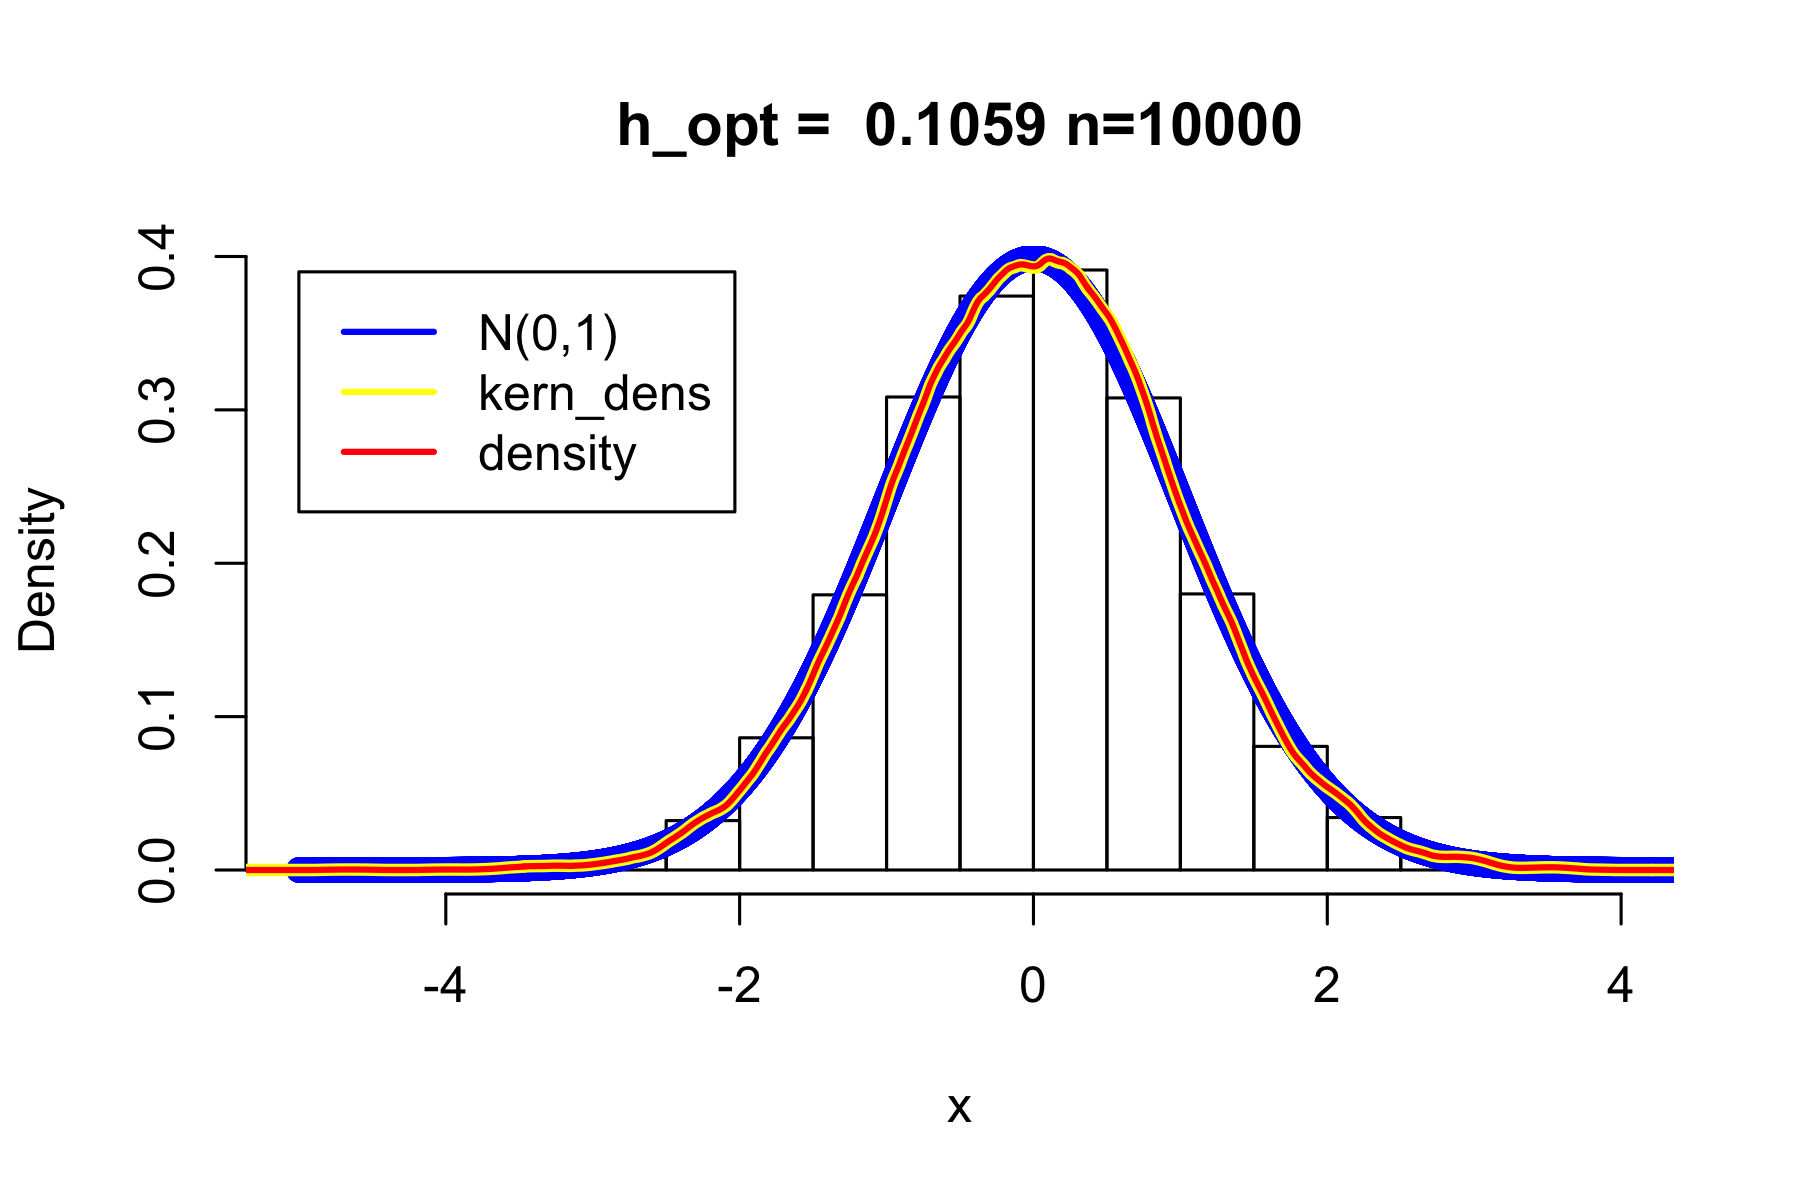
\includegraphics[width=1\linewidth]{../images/stdnorm}
				\caption{Correctness of density estimate}
				\label{fig:stdnorm}
			\end{figure}
		
			\begin{figure}[H]
				\centering
				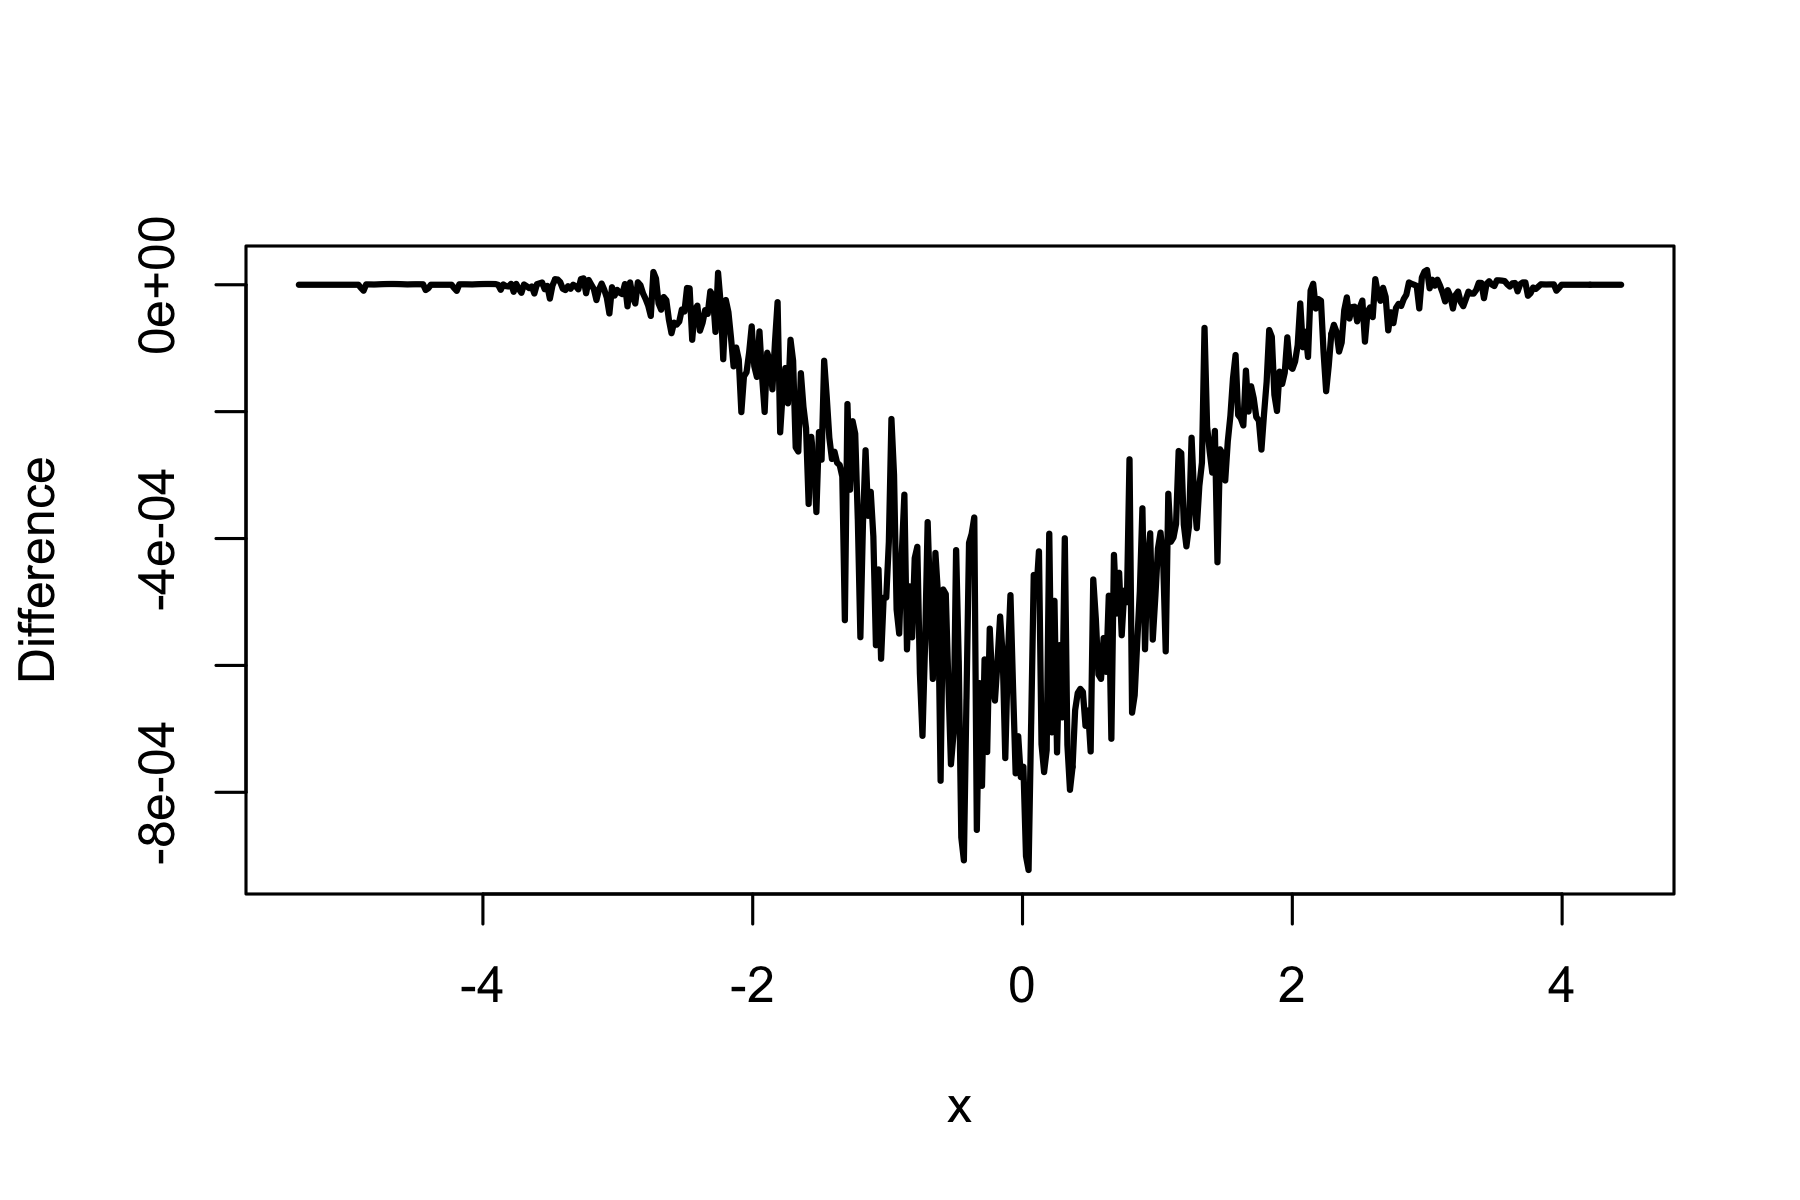
\includegraphics[width=0.7\linewidth]{../images/diff}
				\caption{f\_hat - f\_hat\_dens}
				\label{fig:diff}
			\end{figure}
		\end{column}
	\end{columns}
\end{frame}



%\section{}
%\begin{frame}
%\frametitle{Density benchmark}
%	\begin{columns}
%	\begin{column}{0.48\textwidth}
%		\setlength{\abovecaptionskip}{0pt}
%		\begin{figure}[H]
%			\centering
%			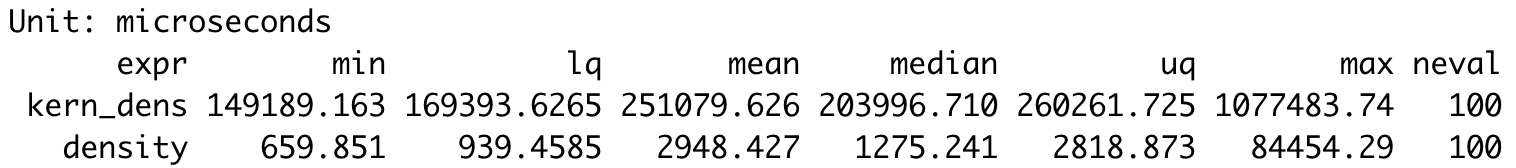
\includegraphics[width=1\linewidth]{../images/dens_bench}
%			\caption{}
%			\label{fig:densbench}
%		\end{figure}
%	\end{column}
%	\begin{column}{0.48\textwidth}
%	
%	\end{column}
%	\end{columns}
%\end{frame}



%Saif
\section{}
\begin{frame}[fragile]
	\frametitle{Bandwidth selection by AMISE}
	\begin{columns}
		\begin{column}{0.48\textwidth}
		\\~\\
			Estimate optimal oracle bandwidth $h_n$ with $\wh{h}_n$:
			\begin{equation}
			\label{eq:07}
				\wh{h}_n = \left( \dfrac{\lVert K \rVert_2^2}{\lVert \wt{f}_0'' \rVert_2^2 \si_K^4} \right)^{\frac{1}{5}} n^{-\frac{1}{5}}
			\end{equation}
			where $\lVert K \rVert_2^2 = \left(\frac{3}{4}\right)^2 \int_{-1}^1 \left(1-x^2\right)^2 \, dx = 0.6$ and\\
			$\sigma _K^2=2 \int_0^1 x^2 K[x] \, dx=2 \int_0^1 \frac{1}{4} 3 x^2 \left(1-x^2\right) \, dx=\frac{1}{5}$
		\\~\\
			Estimate pilot bandwith $r$ with $\wh{r}$:
			\begin{equation}
			\label{eq:08}
				\wh{r} = \left(\dfrac{4}{3}\right)^{\frac{1}{5}} \wt{\si}n^{-\frac{1}{5}} \approx 1.059224 \wt{\si}n^{-\frac{1}{5}}
			\end{equation}
			
			\begin{equation}
			\label{eq:09}
				\begin{aligned}
					\text{IQR}_{\text{theoretical}} &= \Phi^{-1}(0.75) - \Phi^{-1}(0.25)\\
					\text{IQR}_{\text{empirical}} &= \kode{quantile(x, 0.75) - quantile(x, 0.25)}\\
					\wt{\si} &= \min(\wh{\si}, \text{IQR}_{\text{empirical}}/\text{IQR}_{\text{theoretical}})
				\end{aligned}
			\end{equation}
		\end{column}
		\begin{column}{0.48\textwidth}
			\begin{lstlisting}[language=R]
hn_hat <- function(wiggle, n) {
	K_2norm <-0.6
	(25 * K_2norm / wiggle)^(0.2) * n^(-0.2)
}
			\end{lstlisting}
			\begin{lstlisting}[language=R]
r_hat <- function(x, n) {
	sigma_hat <- sd(x)
	IQR <- quantile(x, 0.75) - quantile(x, 0.25)
	IQR_theoretical <- qnorm(0.75) - qnorm(0.25)
	sigma_tilde <- min(sigma_hat, IQR/IQR_theoretical)
	##  Silverman's rule: 0.9 * sigma_tilde * n^(-0.2)
	(4/3)^(1/5) * sigma_tilde * n^(-0.2) ## (4/3)^(1/5) = 1.059224
}
			\end{lstlisting}
		\end{column}
	\end{columns}
\end{frame}



%Martin
\section{}
\begin{frame}[fragile]
	\frametitle{Optimization}
	
		Squared norm of 2nd derivative of pilot density
		\begin{equation}
		\label{eq:10}
			\lVert \wt{f}''\rVert_2^2 = \dfrac{1}{8n^2r^5\sqrt{\pi}} \sum_{i=1}^n \sum_{j=1}^n\left[ e^{c_1z_{ij}^2} \left( (c_2z_{ij})^4 - 6(c_2z_{ij})^2 + 3 \right) \right]
		\end{equation}
	
		Nested
			\begin{lstlisting}[language=R]
wiggle_gauss <- function(x, r) {
wiggle = 0
c1 = -1/(4*r^2)
c2 = 1/(sqrt(2)*r)
for(i in seq_along(x)){
	for(j in seq_along(x)) {
		z <- (x[i] - x[j])/c2
		wiggle <- wiggle + exp(c1 * z^2) * ((c2*z)^4 - 6 * (c2*z)^2 + 3)
	}
}
wiggle <- wiggle / (8 * n^2 * r^5 * sqrt(pi))
wiggle
}
			\end{lstlisting}

\end{frame}

%Martin (cont)
\section{}
\begin{frame}[fragile]
	\frametitle{Optimization (cont)}
	Sum
		\begin{lstlisting}[language=R]
wiggle_gauss_vec <- function(x, r) {
wiggle = 0
c1 = -1/(4*r^2)
c2 = 1/(sqrt(2)*r)
for(i in seq_along(x)){
	z <- (x[i] - x)/c2
	wiggle <- wiggle + sum(exp(c1 * z^2) * ((c2*z)^4 - 6 * (c2*z)^2 + 3))
}
wiggle <- wiggle / (8 * n^2 * r^5 * sqrt(pi))
wiggle
}
	\end{lstlisting}
	Outer
		\begin{lstlisting}[language=R]
wiggle_gauss_outer <- function(x, r) {
c1 = -1/(4*r^2)
c2 = 1/(sqrt(2)*r)
wiggle <- outer(x, x, function(ww, w){
	z <- (ww - w)/c2
	exp(c1 * z^2) * ((c2*z)^4 - 6 * (c2*z)^2 + 3)
})
sum(wiggle) / (8 * n^2 * r^5 * sqrt(pi))
}
		\end{lstlisting}
	
\end{frame}




%Magnus
\section{}
\begin{frame}
	\frametitle{AMISE plug-in profiling}
			Runtime in ms, \kode{n=1000}
			\begin{figure}
				\centering
				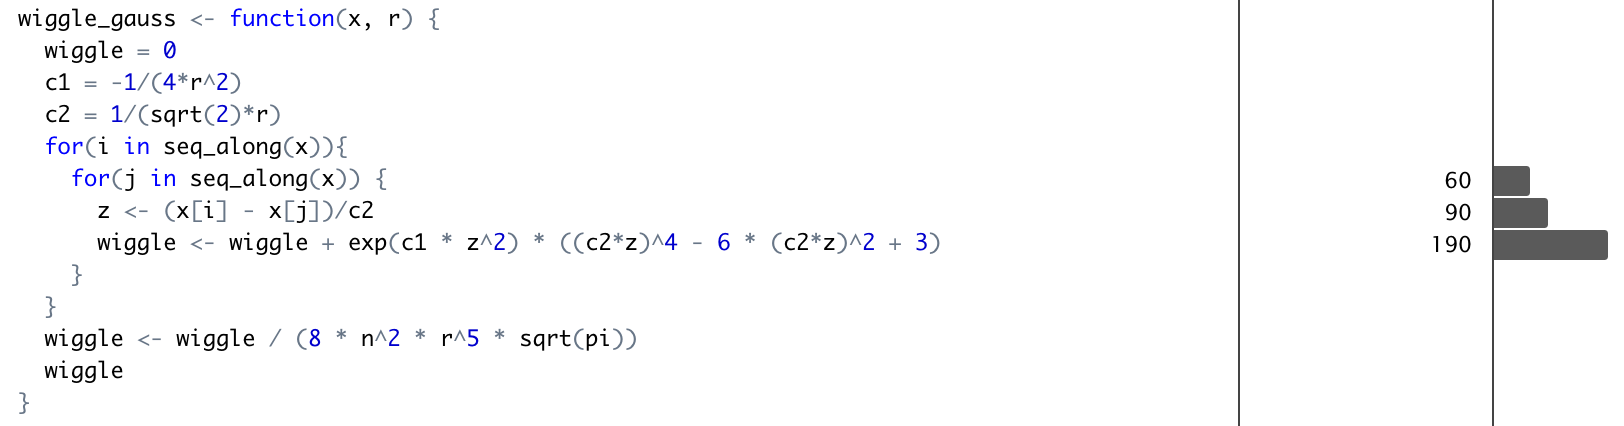
\includegraphics[width=0.7\linewidth]{../images/profile1}
				\caption{$||\wt{f}''||_2^2$ with nested loop implementation}
				\label{fig:profile1}
			\end{figure}
			
			\begin{figure}
				\centering
				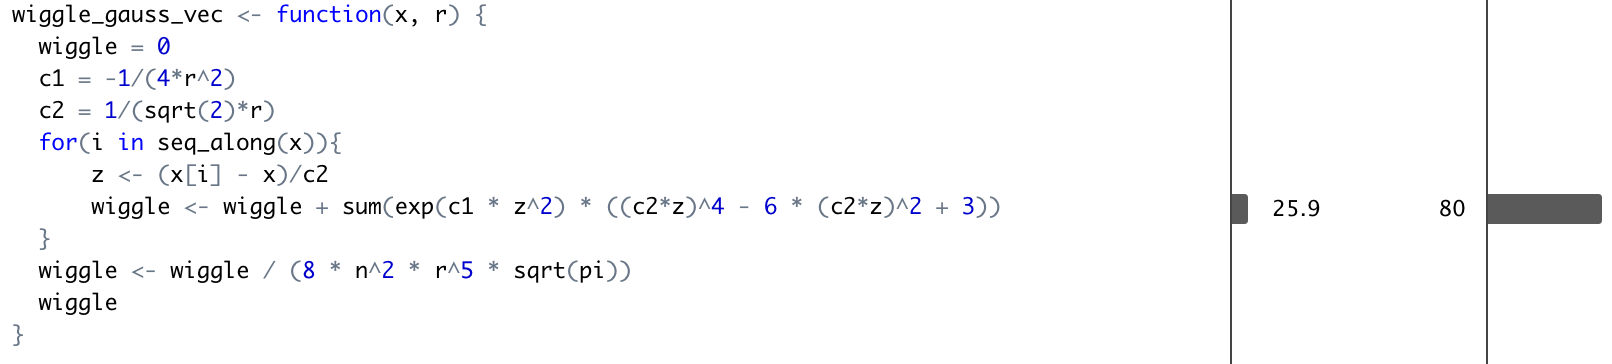
\includegraphics[width=0.7\linewidth]{../images/profile2}
				\caption{$||\wt{f}''||_2^2$ with \kode{sum} vectorization implementation}
				\label{fig:profile2}
			\end{figure}
			
			\begin{figure}
				\centering
				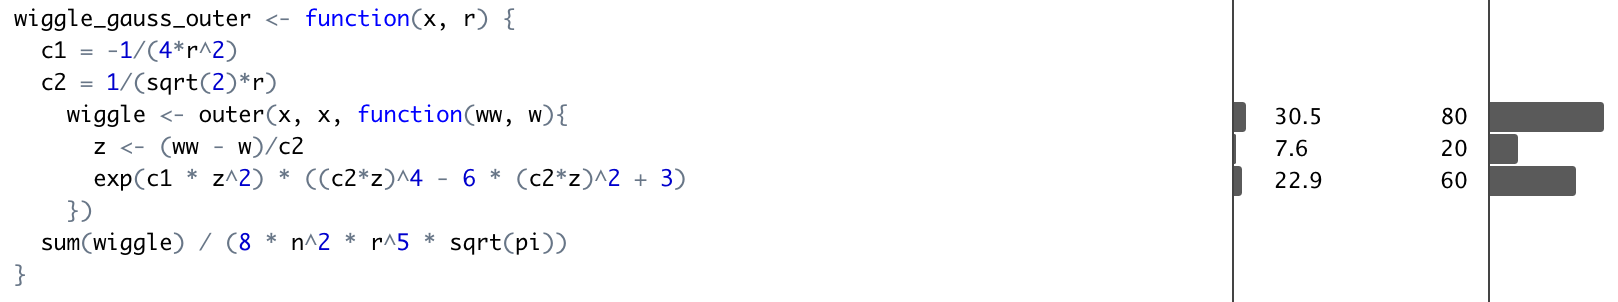
\includegraphics[width=0.7\linewidth]{../images/profile3}
				\caption{$||\wt{f}''||_2^2$ with \kode{outer} implementation}
				\label{fig:profile3}
			\end{figure}
\end{frame}
\note{
	\bls{
		\item profile is not for comparison between functions. It's for internal inspection!
	}
}


%Saif
\section{}
\begin{frame}
	\frametitle{AMISE plug-in benchmarking}
	\begin{columns}
		\begin{column}{0.48\textwidth}
			\setlength{\abovecaptionskip}{-3pt}
			\begin{figure}[H]
				\centering
				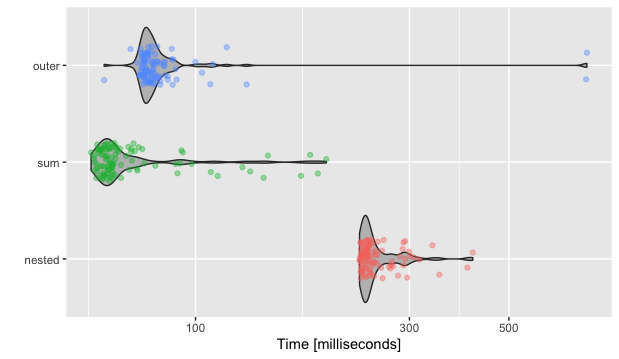
\includegraphics[width=0.95\linewidth]{../images/microbench}
				\caption{n = 1000}
				\label{fig:microbench}
			\end{figure}
			\begin{figure}[H]
				\centering
				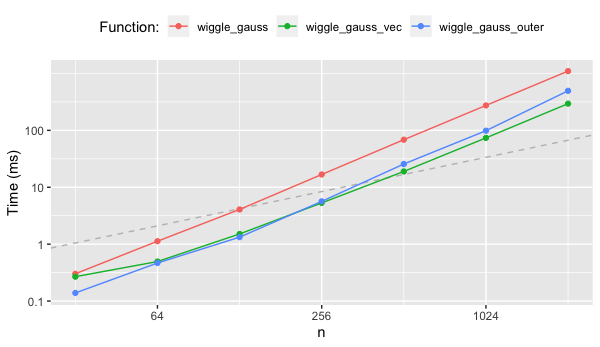
\includegraphics[width=1\linewidth]{../images/runtime_wiggle}
				\caption{}
				\label{fig:runtimewiggle}
			\end{figure}
			Gray dashed line: $o(n)$, \kode{wiggle\_gauss}: $o(n^2)$
		\end{column}
		\begin{column}{0.48\textwidth}
			Runtimes for \kode{kern\_dens} (\kode{my\_density}) and \kode{density}
			\begin{figure}[h]
				\centering
				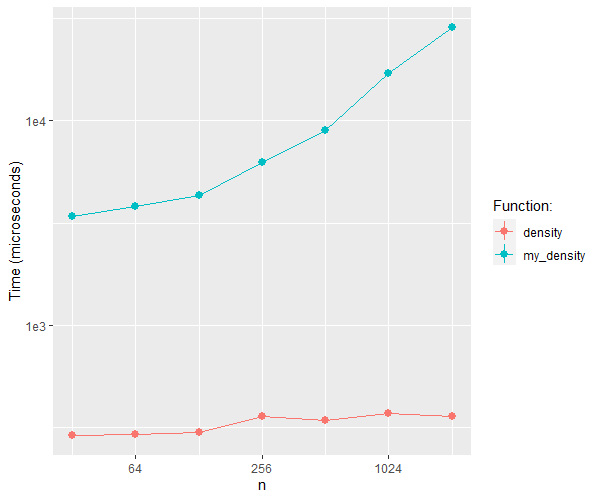
\includegraphics[width=1\linewidth]{../images/runtime_dens}
				\caption{}
				\label{fig:runtimedens}
			\end{figure}
		

			\textbf{Future tests}\\
			\bls{
				\item RCPP for speed
				\item OOP for generality
				\item LOOCV
				\item binning
			}
		\end{column}
	\end{columns}
\end{frame}







\end{document}